\subsection{Infrastructure as Code Approach}
\label{sec:IaC}
Infrastructure as Code (IaC) is a modern DevOps practice that enables the management and provisioning of infrastructure through code instead of manual processes, \parencite[]{RedHat2024InfrastructureAsCode} by using Ansible \parencite[]{RedHat2024Ansible} for configuration management and deployment, vagrant as a testing environment and storing all configuration in version control (github) this is achieved, mocking industry standard production and testing environments.

\subsubsection{Version control (VCS)}
As previously mentioned all configuration files, playbooks and templates are stored in a personal github repository \parencite{ErcModel3_2024OperatingSystems} so the project has:
\begin{itemize}
    \item Change tracking: every change has a valid commit message
    \item Rollback potential: if a mistake is made, I can go back within the repo's history and redeploy working config
    \item The potential for both group members to review/block code changes
    \item Up to date documentation for the state of the firewall
\end{itemize}

\subsubsection{Development workflow and Vagrant}
The coursework brief states that the "Implementation of the coursework should NOT be made on a virtual machine", but nothing about using virtual machines (VMs) for testing, as a real, industry environment would use. As such, using a Vagrant \parencite[]{HashiCorp2024Vagrant} defined VM to run an ARM64 Ubuntu 24.04 (using the net9/ubuntu-24.04-arm64 on an ARM-based dev machine and the ) box mirrored the environment of the 'production' Raspberry Pi (aside from the additional network interface (NIC)). This was defined as figure \ref{code:vagrant-vm-definition}. Vagrant was picked as the program to use as it works as an abstraction layer to define a virtual machine suited for the development environment. The Vagrantfile is Ruby-based, so I could have added automatic checks using Ruby to determine the CPU architecture as I switch between my PC (x86-based Windows/Ubuntu Machine) and my laptop (ARM-based MacBook Air) but I have opted for commenting each line out when it's not being used e.g. \verb|# rasta.vm.box = "net9/ubuntu-24.04-arm64"| when using the cloud (x86) image.

\begin{figure}[H]
    \centering
    \begin{minted}{Ruby}
Vagrant.configure("2") do |config|
    config.vm.define "firewall2-u" do |rasta|
      # rasta.vm.box = "net9/ubuntu-24.04-arm64"
      rasta.vm.box = "cloud-image/ubuntu-24.04"

      rasta.vm.network "private_network", ip: "10.0.1.185"

      rasta.vm.provider "virtualbox" do |v|
        v.memory = 4096
        v.cpus = 2
        v.name = "control1-vagrant"
      end

      rasta.vm.provision "ansible" do |ansible|
        ansible.playbook = "provision.yml"
        ansible.limit = "all"
      end
    end
  end
    \end{minted}
    \caption{The Vagrantfile defining the virtual machine 'firewall2-u' as a testing environment }
    \label{code:vagrant-vm-definition}
\end{figure}

This VM acts as [firewall-test] target in the Ansible inventory, while the physical Pi is the [firewall-prod] at IP 10.0.0.1 as per figure \ref{subsec:ansible}. Combining Ansible, Git(hub) and Vagrant ensures:
\begin{itemize}
    \item Safe experimentation: Any rules created can be tested before pushing them to the real Firewall
    \item Continuous Integration \parencite{IBM2024CICDPipeline}: as both students can push code to their respective VM
    \item Additional snapshots/rollbacks: VirtualBox snapshots allow instant restoration of the VM should bad config get pushed
\end{itemize}

This implementation follows the development flow of figure \ref{fig:dev-workflow}
\begin{figure}[H]
    \centering
    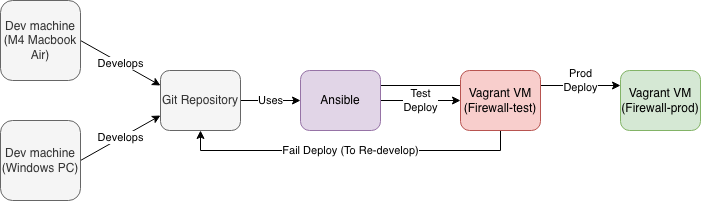
\includegraphics[width=0.8\linewidth]{Diagrams/os-dev-workflow.drawio.png}
    \caption{A diagram showing a high-level breakdown of the development workflow from dev machine to firewall instead of working just on the Pi and losing everything should a mistake arise}
    \label{fig:dev-workflow}
\end{figure}

\subsubsection{Configuration Management with Ansible}
Ansible is one of the most common open-source configuration management tools \parencite[]{OpenSource2018ConfigurationManagement}, it was selected as its:
\begin{itemize}
    \item Agentless: Less overhead on the Raspberry Pi as all work is done on the development machine and uses SSH to deploy files
    \item Idempotency: Playbooks can be run over and over and won't change anything unless there's a change to the codebase
    \item Comprised of easily-readable YAML playbooks
\end{itemize}

\paragraph{Playbook Structure - provision.yml}
\label{sec:provision.yml}
Each playbook/role has a definition and an endgoal. The \verb|provision.yml| playbook is attached to the \verb|vagrantfile| so it provisions the vm, it also provisions the Raspberry Pi.

NEEDS REFERENCE

\paragraph{Playbook Structure - netplan.yml}
\label{sec:netplan.yml}
To adhere to Ansible best practices \parencite{Ansible2024RoleReuse}, playbooks are all defined using the Role definition using a main YAML file that will call the role, figure \ref{code:ansible-netplan-role} shows the netplan role.

\begin{figure}[H]
    \centering
    \begin{minted}{YAML}

    \end{minted}
    \caption{The playbook used to deploy the netplan config to the test (and production) firewalls using Ansible facts}
    \label{code:ansible-netplan-role}
\end{figure}

\paragraph{Playbook Structure - iptables.yml}
\label{sec:iptables.yml}

TODO - REWRITE THIS PARAGRAPH
To adhere to Ansible best practices \parencite{Ansible2024RoleReuse}, playbooks are all defined using the Role definition using a main YAML file that will call the role.

\begin{figure}[H]
    \centering
    \begin{minted}{YAML}
---
- name: Install and deploy firewall
  hosts: firewall-test
  become: yes
  roles:
    - iptables
    \end{minted}
    \caption{The playbook used to deploy the Iptables config to the test (and production) firewall}
    \label{code:ansible-iptables-role}
\end{figure}

\begin{figure}[H]
    \centering
    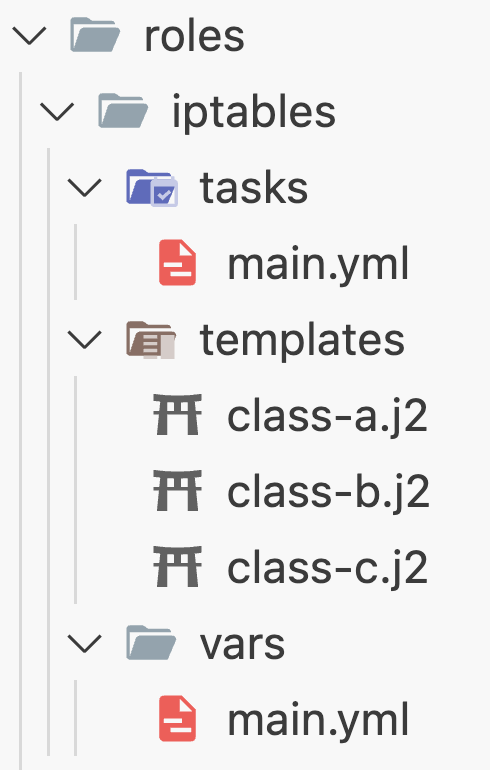
\includegraphics[width=0.3\linewidth]{Report_Images/os-iptables-role.png}
    \caption{The iptables Ansible role structure following best-practice}
    \label{screenshot:ansible-iptables-role}
\end{figure}

The main playbook (iptables.yml shown in figure \ref{code:ansible-iptables-role}) sets up and deploys the config to the testing firewall and the production firewall (when 'test' is substituted with 'prod'). Figure \ref{screenshot:ansible-iptables-role} shows the rest of the role the \verb|iptables.yml| playbook calls, namely the tasks file in \verb|tasks/main.yml| file in figure \ref{code:ansible-iptables-tasks}.

\begin{figure}[H]
    \centering
    \begin{minted}{YAML}
---
- name: Install iptables-persistent
  apt:
    name:
      - iptables-persistent
    update_cache: yes

- name: Create config directory
  file:
    dest: /etc/iptables/
    state: directory
    mode: '0664'

- name: Deploy iptables configs
  template:
    src: "{{ item }}.j2"
    dest: /etc/iptables/{{ item }}
  loop:
    - class-a
    - class-b
    - class-c
  
- name: Apply iptables configs
  command: iptables-save > {{ item }}
    \end{minted}
    \caption{The tasks file used to carry out the iptables deployment}
    \label{code:ansible-iptables-tasks}
\end{figure}

The tasks file:
\begin{itemize}
    \item Installs iptables-persistent package
    \item Creates the /etc/iptables directory
    \item Renders a Jinja2 template for each network zone as defined in \ref{} TO DO REFERENCE.
\end{itemize}